\documentclass{article}
\usepackage{graphicx}
\usepackage{titling}  % For custom title page
\usepackage{circuitikz}
\usepackage{amsmath}
\usepackage{amssymb}
\usepackage{booktabs,tabu}
\usepackage{float}

\title{Experiment 1: Basic Filter Design}
\author{Samyak Sheersh, Aryam Shankar}
\date{06 August 2024}
\newcommand{\subtitle}[1]{%
  \posttitle{%
    \par\end{center}
    \begin{center}\large#1\end{center}
    \vskip0.5em}%
}

\begin{document}

% Custom title page
\begin{titlepage}
    \centering
    
\includegraphics[width=0.2\textwidth]{KGP_logo.png}\par\vspace{1cm}
    {\scshape\LARGE Department of Electronics and Electrical Communication Engineering, IIT Kharagpur\par}
    \vspace{1cm}
    {\huge\bfseries Experiment 3:  Dual Tone Multifrequency Coder/Decoder\par}
    \vspace{1.5cm}
    {\Large\itshape Samyak Sheersh \par}
    \vfill
    % Identifying information at the bottom
    {\large Roll Number: 22EC30045\par}
    {\large Group Number: 24\par}
    \vfill
    {\large \today \par}
\end{titlepage}

\section{Tasks}
\begin{enumerate}
    \item Design a DTMF using a digital filter in MATLAB
    \item Simulate a random signal(emulating key presses from a user) and then decode it using the DTMF decoder
    \item Simulate non idealities of the conducting medium by introducing a squared dependency and random noise and check the accuracy of the decoding system.
\end{enumerate}

\section{Procedure and Results}
\subsection{Task 1}
We choose $f_l$ from the list $[697, 770,852,941]$ and  $f_h$ from the list $[1209, 1336, 1477, 1633]$, which will generate a signal composed of the two frequencies representing the character that we just pressed, 

We decode this signal using a series of $L$-point band-pass filter, centered around each of the frequencies mentioned above: 
\begin{equation}
  h[n]=\beta \cos(\omega_c n)\ \forall 0 \leq n \leq L
\end{equation}

As we increase $L$, the bandwidth becomes narrower, and $\beta$ can be used to cadjust gain of the signal passing through the filter. 

We decoded the individual frequencies by convolving the given signal and $h[n]$, we then saw which convolution sequence had the maximum value (since if the signal contains $\omega_c$, the signal would be more aligned to $\cos(\omega_c n)$, and thus the convolution would achieve a greater maximal value)

\subsection{Task 2}
The task here was simply applying the method we developed above to a time signal which includes multiple key presses, and thus would have different sets of frequencies at different points of time.

We decoded the whole signal by splicing it by detecting extend periods of time when the signal is 0(we chose $\Delta n\geq 20$), and then applied the algorithm described in Task 1 on each of the segments obtained. 

\begin{figure}[!ht]
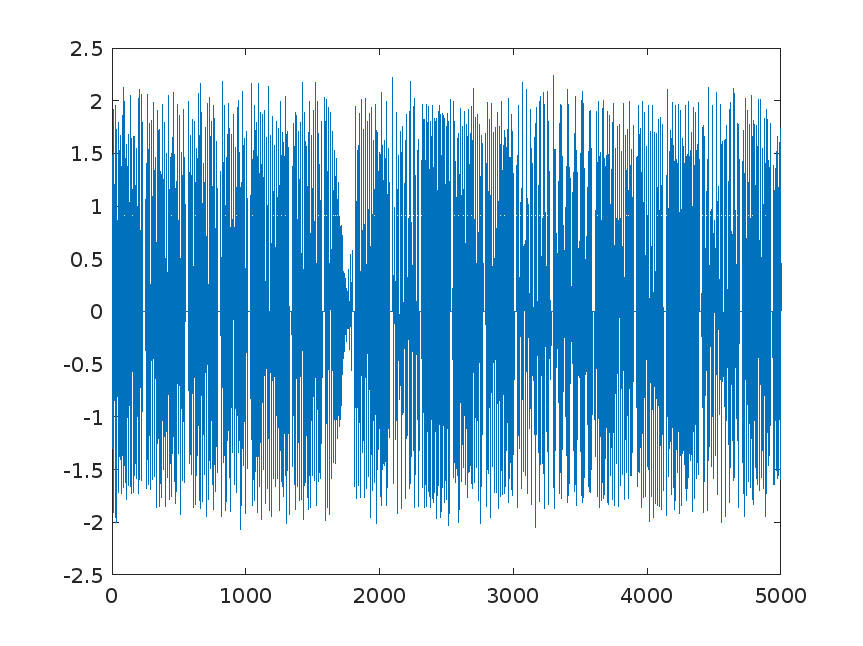
\includegraphics[width=\textwidth]{signal_for_message.png}
\caption{Signal which encoded the message $``56\#62\#31AC\#2A712\*A\#C"$}
\label{fig:signal}
\end{figure}
\clearpage
\subsection{Task 3}
Here, we needed to simulate a non-ideal channel which would introduce a squared dependency and random noise to the signal. Thus the signal we generated $x[n]$ now becomes:
\begin{equation}
  x_f[n]=x[n]+Ax^2[n]+\epsilon[n]
\end{equation}

where A is the strength of distortion and $\epsilon \sim N(0,\sigma^2)$, where $\sigma^2$ is variance for the random noise.


To test the resillience of the system we:
\begin{enumerate}
  \item varied A from 0 to 10, and then varied $\sigma$ from 0.1 to 10, thus distorting the signal to various different levels. 
  \item We then generated a 100 random signals keeping A and $\sigma$ the same, and running the algorithm, on each of them, comparing the decoded and the original message sequence. 
  \item We used a pass fail to test the accuracy in the above system i.e. if even one character differs between the decoded and the original signal, the attempt is considered wrong. 
  \item We then plotted the heatmap (ref. Figure \ref{fig:heatmap}) 
\end{enumerate}

\begin{figure}[!ht]
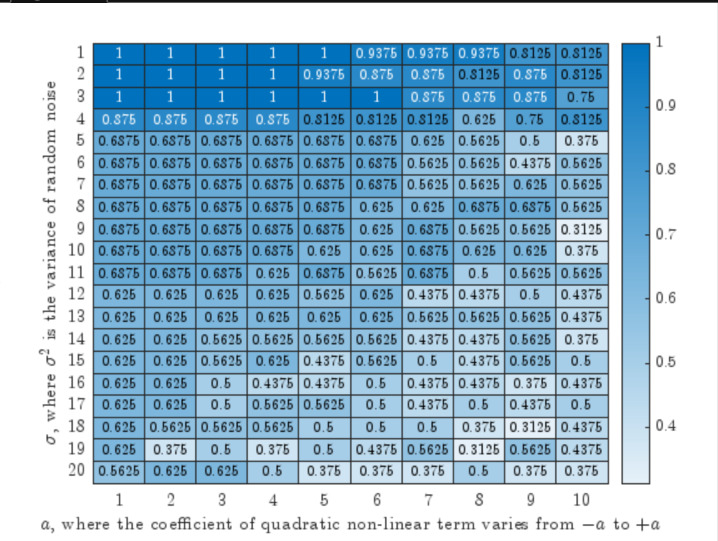
\includegraphics[width=\textwidth]{heatmap.jpeg}
\caption{Heatmap for Task 3}
\label{fig:heatmap}
\end{figure}
\clearpage
\section{Discussion}
\subsection{Samyak Sheersh, 22EC30045}
\begin{enumerate}
  \item We use the sets of frequencies given above since they do not have overlapping harmonics and the sums of any two frequencies doesn't add up to a third one. This means that even in a non-linear channel, frequencies won't overlap, and thus the message will be much less likely to be muddled and that unwanted frequencies won't be detected at the reciever.
  \item As we explained in the Procedure section for Task 1, the algorithm that we used did not need to normalise the convolution, but we found that at $\beta=0.017$ the values of the convolved signal were normalised between 0 and 1 
  \item As we can see in the heatmap in Figure \ref{fig:heatmap}, the accuracy of the algorithm decreases as the strength of the noise and the non-linearities increase. Although, it decreases faster as $\sigma^2$ increases in comparison  to A, which is expected as even the non-linearities won't be detected by our filters (since the harmonics and sums of frequencies won't be detected as we explained in point 1). 
  \item We also had to ensure that the segments of the signal with distinct frequencies (see Figure \ref{fig:signal}, the lobes between areas where the signal is 0) were at least 3 times the length of the filter (i.e. $3L$), which is again expected since, we become more sure about the constituent frequencies in a signal the longer it persists(see Heisenberg's uncertanity principle). 

\end{enumerate}
\end{document}
